\documentclass[10pt,a4paper]{article}

\usepackage[a4paper,hmargin=2.5cm,vmargin=3cm] {geometry}
\usepackage{fix-cm}
\usepackage{amsmath,amssymb,amsthm}
\usepackage{tikz}
\usepackage{graphicx}
\usepackage[polish,english]{babel}
\usepackage[T1]{fontenc}
\usepackage[utf8]{inputenc}
\usepackage{url}
\usepackage{verbatim}
\usepackage{color}
\usepackage{ae}
\usepackage[ruled]{algorithm}
\usepackage{algorithmicx}
\usepackage{algpseudocode}
\usepackage[breaklinks]{hyperref}
\usepackage[polish,english]{babel}
\usepackage{multirow}
\usepackage{epstopdf}
\usepackage{listings}

\newtheorem{theorem}{Theorem}
\newtheorem{lemma}{Lemma}

\definecolor{myRed}{rgb}{0.9,0.3,0.1}
\newcommand{\pawel}[1]{\noindent\colorbox{myRed}{Pawel: #1}}
\definecolor{myYellow}{rgb}{0.99,0.99,0.05}
\newcommand{\jarek}[1]{\noindent\colorbox{myYellow}{Jarek: #1}}
\newcommand{\todo}[1]{\noindent\colorbox{myRed}{TODO: #1}}

\newcommand{\Oh}{\mathcal{O}}

\begin{document}

%%%%%%%%%%%%%%%%%%%%%%%%%%%%%%%%%%%%%%%%%%%%%%%%%%

\pagenumbering{roman}

\topmargin-20pt
\oddsidemargin0pt
\evensidemargin0pt
\textheight660pt
\textwidth445pt

\selectlanguage{polish}
\begin{titlepage}
\Large

\begin{center}

\textbf{\large%
Uniwersytet Wrocławski\\
Wydział Matematyki i Informatyki\\
Instytut Informatyki}


\vspace{4cm}
Jarosław Gomułka [DRAFT]

\vspace{0.5cm}
\textbf{%\normalsize%
Shuffla: fast and scalable full-text search engine}

\end{center}

\vspace{7cm}
\begin{flushright}
\begin{minipage}[c]{6.2cm}
  Praca magisterska\\
  napisana pod kierunkiem\\
  dr. Pawła Gawrychowskiego
\end{minipage}
\end{flushright}

\vfill

\begin{center}
 Wrocław 2012
\end{center}

\newpage

\end{titlepage}

\newpage

\thispagestyle{empty}

\Large

~\vfill
Oświadczam, że pracę magisterską wykonałem samodzielnie i zgłaszam ją do oceny.

\vspace{2cm}
Data: \dotfill\quad Podpis autora pracy: \dotfill


\vspace{4cm}
Oświadczam, że praca jest gotowa do oceny przez recenzenta.

\vspace{2cm}
Data: \dotfill\quad Podpis opiekuna pracy: \dotfill

\normalsize

\restoregeometry
%%%%%%%%%%%%%%%%%%%%%%%%%%%%%%%%%%%%%%%%%%%%%%%%%%

\newpage
\thispagestyle{empty}

\begin{abstract}
Celem tej pracy jest stworzenie efektywnego i skalowalnego narzędzia do dokładnego przeszukiwania zbioru użytkowników dużego portalu społecznościowego. Przechowane dane to imię, nazwisko, wiek, oraz miejsce zamieszkania.

Użytkownik portalu może wyszukiwać innych użytkowników poprzez:
\bigskip
\begin{enumerate}
\item{podanie imienia (jego prefiksu lub podsłowa),}
\item{podanie nazwiska (jego prefiksu lub podsłowa),}
\item{podanie wieku (dokładnie bądź przez określenie dolnej i górnej granicy),}
\item{podanie miejsca zamieszkania (jego prefiksu lub podsłowa).}
\end{enumerate}

\bigskip

Kolejnym założeniem jest konieczność personalizacji wyników wyszukiwania. Na przykładu użytkownik z San Francisco szukający Jane powinien dostać w pierwszej kolejności osoby o imieniu Jane z San Francisco, następnie osoby z Kaliforni, Stanów Zjednoczonych, a dopiero na samym końcu z innych części świata.

Jednym z możliwych rozwiązań tak postawionego problemu jest zastosowanie jednej z popularnych relacyjnych baz danych. Inną możliwością jest użycie wyszukiwarki tekstowej takiej jak Apache Solr czy Sphinx Search. Jeszcze innym pomysłem jest zaimplementowanie własnego narzędzia. Celem tej pracy jest przedstawienie Shuffli, wyspecjalizowanej wyszukiwarki stworzonej przeze mnie z myślą o tym konkretnym problemie. Oprócz przedstawienia architektury i szczegółów implementacji, porównam jej efektywność z PostgreSQL, Apache Solr, Sphinx Search.

\bigskip
Pracuję nad portalem nk.pl (który jest największym polskim portalem społecznościowym) od początku roku 2011. W sierpniu 2011 roku zostało mi powierzone rozwiązanie tego problemu.

\bigskip
\noindent \textbf{Słowa kluczowe:} bazy danych, nosql
\end{abstract}

\selectlanguage{english}
%%%%%%%%%%%%%%%%%%%%%%%%%%%%%%%%%%%%%%%%%%%%%%%%%%


\title{Shuffla: fast and scalable full-text search engine}
\author{Jarosław Gomułka}

\maketitle

\begin{abstract}
Given a list of people (their first name, last name, age, home town) we want to provide high-available, scalable and very fast solution that can search through such data.
User can narrow search results by:

\bigskip
\begin{enumerate}
\item{defining first name (its prefix or substring)}
\item{defining last name (its prefix or substring)}
\item{narrowing age (user can provide lower or/and upper bound for age)}
\item{defining city (its prefix or substring)}
\end{enumerate}

\bigskip
It would be great if results could be personalized. For example, if user from San Francisco is looking for Jane, top results should show Jane's from San Francisco, then Jane's from California, then rest of U.S. One of possible solution is to use relational database. Other solution is to use full-text search engine like Apache Solr or Sphinx Search. Another solution is to develop very own search engine dedicated to solving such task. In this paper I will describe Shuffla, full-text search engine created by me. I will compare it to Sphinx, Solr, PostgreSQL. 

\bigskip
I'm working on nk.pl (which is biggest polish social networking website) since the beginning of 2011. In August 2011 I was appointed to solve the task described above. 

\bigskip
\noindent \textbf{Keywords:} database, nosql
\end{abstract}

\pagenumbering{arabic}
%%%%%%%%%%%%%%%%%%%%%%%%%%%%%%%%%%%%%%%%%%%%%%%%%%

\section{Problem definition}

Lets define table definition by combination of
\begin{enumerate}
\item table name
\item list of pairs <column name, type of column>
\end{enumerate}
Type of column can be either string or number

\subsection{Selecting data}
There are different possible conditions for different types. Possible conditions for numbers are comparisons, inequalities and strict inequalities. Strings are compared using lexicographic order, so comparisons, inequalities and strict inequalities should be supported. There are two additional conditions
\begin{enumerate}
\item Checking if given string is prefix of value of selected column. 
\item Checking if given string is substring of value of selected column. 
\end{enumerate}
Presenting results:
\begin{enumerate}
\item User can define order in which results will be returned.
\item User can narrow number of results by defining offset and 
limit
\end{enumerate}

Narrowing result described in abstract is possible with defined model. Personalizing results can be done by mapping cities to GPS coordinates. GPS coordinates can be added to scheme. For selecting users in some range we can add conditions   
\begin{enumerate}
\item{someLatitiude - radius $\leq$ latitude $\wedge$ latitude $\geq$ someLatitude + radius}
\item{someLongitude - radius $\leq$ longitude $\wedge$ longitude $\geq$ someLongitude + radius}
\end{enumerate}

\section{Shuffla's competition}
Problem described in this paper is solvable by various existing software. There are two most common kinds of software which can be used:

\subsection{Relational databases}
In these paper I'm only testing PostgreSQL which is considered best RDBMs nowadays \todo{source do tego fajnego artykułu z reddita}.

\subsubsection{PostgreSQL}
PostgreSQL has really cool features like: real time index creation, geospatial index \todo{Uzupełnij to}. PostgreSQL implements replication (\todo{what kinds}), slow log, error log, it's performance can be easily overlooked \todo{to chyba zle slowo} by monitoring software like munin, new relic \todo{Jak to działa}. SQL implies very strong typing system. PostgreSQL processes comparisons and inequalities very fast as long as proper indexes are created. Big disadvantage of using PostgreSQL for this problem is performance on substring queries. B-tree based indexes are not supporting fast processing of substring queries. There are attempts to create full-text indexes (gist, gin) which could outperform classical index based on B-tree. \todo{Opisz jak wygląda persistence}. Example of processing query by B-tree: \verb|first name = John| $\wedge$ \verb|substring(last name) = qwertyabc| $\wedge$ \verb|limit 1|. In this case engine is finding first person with first name John. It takes $O(\log n)$ time. Finding another person with first name John takes $\Oh(1)$. Unfortunately all these rows must be processed one by one for checking if they contain substring \verb|qwertyabc|. Since there is no one with such name, engine will process all guys named John, and it will find nothing.

\subsection{Full-text search engine}
Another solution is to use full-text search engine. The most popular full-text search engines are Sphinx search and Lucene Solr. Almost all big players are choosing Sphinx and Solr over others such as Elastic Search, \todo{Nie pamiętam tych 2 nazw już} so I'm going to consider only these two. Both engines are based on similar data structure called inverted index. Inverted index keeps list of every occuring word in database. For each word inverted index remembers where this word occurs. This is similar to glossaries which we can often see at the end of books. Such inverted index is stored on disk. When processing query, engine selects best strategy to follow. Strategy can be \todo{english na postrzegana} as procedure
\begin{enumerate}
\item Narrow words from inverted index which need to be process as much as possible. 
\item Process remaining words. 
\end{enumerate}
For example if query is \verb|first name = John| $\wedge$ \verb|limit 1| then we are only interested in word John from inverted index. Engine finds first occurence and returns it. If query is \verb|first name = John| $\wedge$ \verb|substring(last name) = qwertyabc| $\wedge$ \verb|limit 1| then it is likely that there are more Johns then all people with last name containing \verb|qwertyabc|. Engine could use suffix tree which contains all words from inverted index. It would find that there is nobody with such last name. Such output would be rendered very fast, probably even without reading inverted index. In worst case scenario algorithm works in linear time. Example for such a case could be \verb|substring(last name)=a| $\wedge$ \verb|substring(last name) = b| $\wedge$ ... $\wedge$ \verb|substring(last name) = z| $\wedge$ \verb|limit 1|. Almost whole inverted index must be processed but still result set will be empty.

\subsubsection{Solr}

Solr is a popular open source search platform from the Apache Lucene project. It has lots of very cool features like faceted searches, geospatial searches, string tokenizers (makes John and Johnny to be interpreted as the same name). It is easily extendable for new features. Solr implements master-slave replication which solves scalability problems. Everything is perfect except one thing. 

Solr doesn't modify database in real-time. Data isn't added immediately to database after insert/update commands. Data is actually inserted after calling commit command. Commit is very costly operation because it requires all caches to be invalidated. Even for table with few entries, commit takes more than 0.1 sec. Time for commit grows with growing size of data. Instance of Solr in nk contains 40 million entries and commit takes about 20 seconds. Commit doesn't block database which is very important. After commit, search engine is in warming stage. It means that all caches are flushed, so first queries can run slowly. After number of processed queries, engine is past warming stage and queries are handled much faster.

There is a rumour that twitter was able to modify source of Solr so they could have real-time modifications (apparently they succeeded, source needed).

\subsubsection{Sphinx search}

\todo{Ficzery solra}

In nk we were really close to choosing Sphinx search over Solr. We didn't choose Sphinx because it doesn't have replication. It was the only reason.
There is a way to simulate replication. Inverted index is stored on disk. Directory containing index could be replicated by filesystem (for example NFS \todo{source, dowiedz się co się dzieje gdy padnie master w nfsie}). But if index is big than syncing such directories would take too much time and would be inefficient and problematic.

There are several high-traffic websites with Sphinx search. They horizontally partition searched data across search nodes and then process it in parallel \cite{SPHINXPARAL}.

Replication is very important to us because in case of server failure we want to avoid downtime. So it was kind a deal breaker for us. I'm considering sphinx search in this paper because maybe some day they are going to implement some kind of replication.

Except of replication sphinx has another problem. There are two different kinds of indexes in sphinx.
\begin{enumerate}
\item Real-time index - enables inserts
\item Normal index - modifications possible only by rebuilding whole index
\end{enumerate}

Real-time index has many caveats \cite{SPHINXCAV}. Prefix and substring queries are not supported yet. Periodical rebuild of index with more than 40 million elements is problematic. Apache Solr and Sphinx search are using similar data structures. Since capabilities and number of features of Solr are much greater I decided to look only into Solr. 

\bigskip
It seems that none of existing solutions are processing search queries very fast. In worst case scenario it's always $\Oh(n)$. All solutions are working on data stored on disk. In age when RAM is cheap and servers with +32GB RAM are considered average solutions working in RAM memory are \todo{english na mile widziane}. Although data stored on disk could be transfer to RAM by ramdisks, it shows that such solution isn't primary target to software creators. For me it seems that this area has room for improvement. That's why I decided to create my own search engine.  

\section{Algorithm description}
We can clearly see analogy to multidimensional range searches. All conditions (except substring condition) can be represented as half-plane (or half-planes) which narrows the search space. There are three data structures for performing efficient searches in a multidimensional space:

\begin{enumerate}
\item Range Tree \cite{CGAAA}
\item Inverted Index \cite{CGAAA}
\item K-D tree \cite{CGAAA}
\end{enumerate}

Complexities (where $d>=2$)

\begin{tabular}{|l|c|c|c|c|}
\hline Algorithm & Insert (without balancing) & Delete (without balancing) & Search & Space \\
\hline K-D tree & $\Oh(\log{n})$ & $\Oh(\log{n})$ & $\Oh(n^{1-1/d} + k)$ & $\Oh(n)$ \\
\hline Inverted index & $\Oh(\log n)$ & $\Oh(\log n)$ & $\Oh(n)$ & $\Oh(n)$ \\
\hline Range tree & $\Oh(\log^{d-1}{n})$ & $\Oh(\log^{d-1}{n})$ & $\Oh(\log^d{n})$ & $\Oh(n\log^{d-1}{n})$ \\
\hline 
\end{tabular}

\bigskip

Since both Solr and Sphinx are using inverted index I decided not to follow this direction and try something new. It seems that K-D tree could outperform inverted index on search queries.

I chose to implement K-D trees over Range trees because:
\begin{enumerate}
\item They are only worse in processing search requests. Operations which modify data i.e. insert/delete are more important. If they are very fast, scaling can be easily achieved (for example by implementing master-slave replication). Moreover, while the search bounds are worse in theory, they seem to be significantly better in practice.
\item Space complexity of range trees is unacceptable for this kind of problem. With 5 columns and 10 million rows, algorithm would require more than 100GB of RAM.
\end{enumerate}

\bigskip
We also have queries with substring conditions. In each node of K-D tree we could store structure which efficiently process substring queries. We could use suffix trees, for example Ukonnen's algorithm \cite{STUKK} .

Complexities:
\begin{enumerate}
\item Adding text to tree: $\Oh(|text|)$
\item Removing text from tree $\Oh(|text|)$
\item Searching text in tree $\Oh(|text|)$
\end{enumerate}

Unfortunately adding linear structure to every node of K-D tree increases the space complexity to $\Oh(n \log n)$

\section{Implementation}

\subsection{HTTP Service}


 (Figure~\ref{fig:httpservice}).

\begin{figure}
\centering
  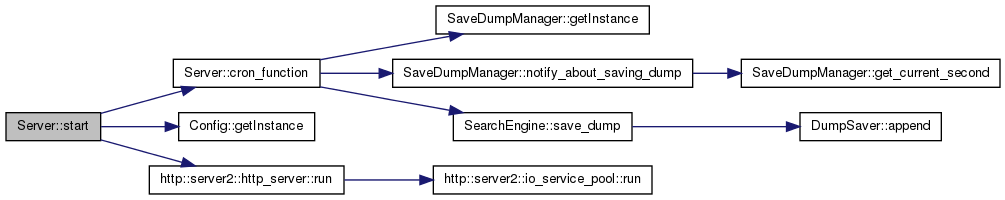
\includegraphics[width=16cm]{start}
  \caption{Processing request begins}
  \label{fig:httpservice}
\end{figure}

I decided that it would be best if search engine could mimic RESTful service. Every search/insert/delete request should be sent as a HTTP request. Server works in the multi-threaded environment. As a base I used \verb|example2| \cite{ASIOHTTP} from \verb|boost::asio| documentation which fulfills my requirements. \todo{Jak działa example2, pula wątków} There is another thread for periodical functions. Currently its invoking only saving snapshots.

 (Figure~\ref{fig:passing}).

\subsection{Validation and passing queries to SearchEngine class}

\begin{figure}
\centering
  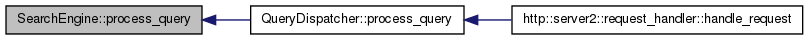
\includegraphics[width=16cm]{passingtosearchengine}
  \caption{Passing control to SearchEngine class}
  \label{fig:passing}
\end{figure}

\verb|http::server2::request_handler::handle_request| passes requesting url to \verb|QueryDispatcher|. QueryDispatcher converts every request to corresponding class by using \verb|QueryCreate|. For example, search request is converted to \verb|SearchQuery|, insert is converted \verb|InsertQuery|, and so on. At this level, syntax validation is performed. In case of an error, HTTP error code 400 is returned, and error message is appended to the log file with errors. 

Instances of query classes are sent to \verb|SearchEngine| class. \verb|SearchEngine| class is responsible for:
\begin{enumerate}
\item data validation (types, correspondence to table definition),
\item measuring running time (slow log purpose),
\item locking tables in case of modifying query,
\item passing valid requests to K-D Trees.
\end{enumerate}

\subsection{Processing insert/delete requests}

Inserting/deleting without tree balancing is pretty straight-forward. Just simple recursion. Balancing is a little bit tricky. 

 (Figure~\ref{fig:rebuild}).

\begin{figure}
\centering
  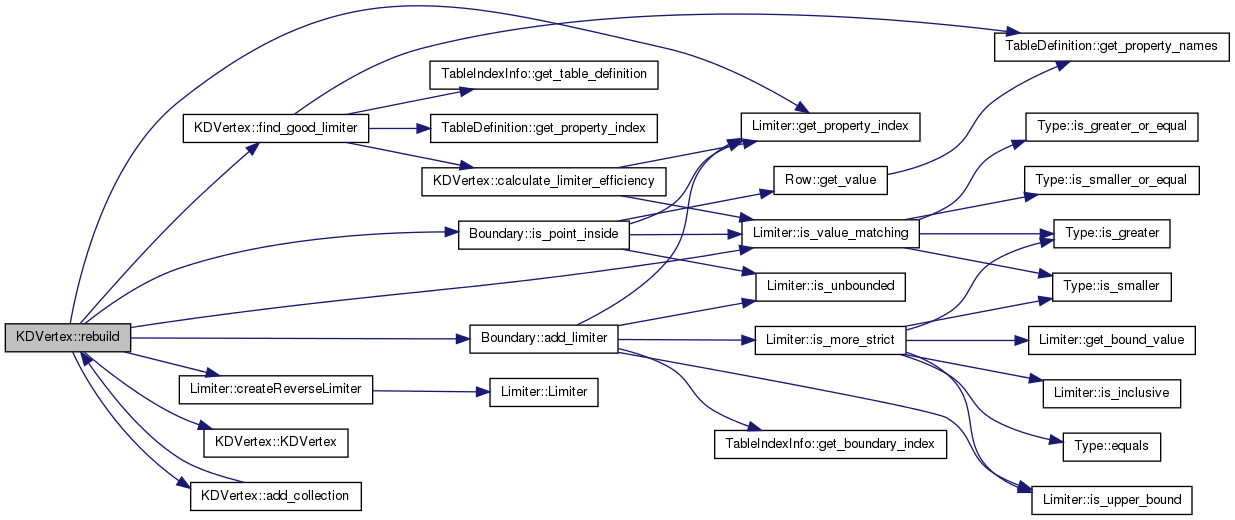
\includegraphics[width=16cm]{rebuild}
  \caption{Rebuilding process}
  \label{fig:rebuild}
\end{figure}

Balancing can be done using any linear algorithm for finding median in set. I've decided to take different approach. In \verb|KDVertex::fing_good_limiter| I'm selecting randomly about 30 rows belonging to node and I'm iterating over them. Based on current coordinate value in this row I'm creating Limiter. \verb|Limiter| is simple class which takes \verb|Row| and \verb|property_name|. For any \verb|Row| limiter can check if given Row satisfy condition defined inside \verb|Limiter|. Algorithm iterates over all rows in node and in linear time calculates limiter efficiency. If limiter efficiency is good enough (See definition of well-balanced tree) than I'm stopping calculations. I've got \todo{Jak ładnie nazwać element podziału} and I'm recursively rebuilding two subtrees. I've decided for this solution because of space efficiency which is $\Oh(1)$. Space complexity is crucial because if it reach linear size, than during rebuilding root, memory usage could double. Such behaviour is very unwelcome in server environment. Implemented solution is $\Oh(n^2)$ but in average case it works well because $\frac{1}{3}$ of elements are creating good limiters.

\subsection{Processing search requests}

 (Figure~\ref{fig:search}).

\begin{figure}
\centering
  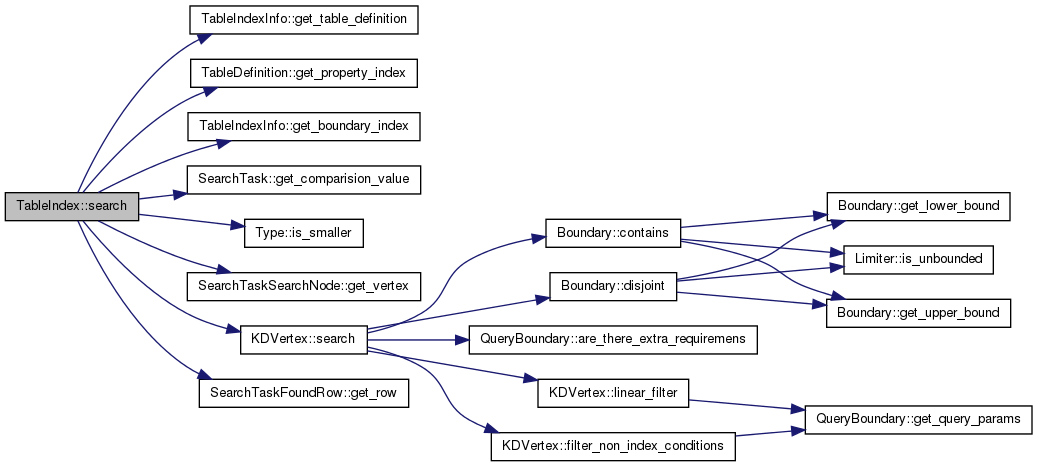
\includegraphics[width=16cm]{search}
  \caption{Processing search request}
  \label{fig:search}
\end{figure}

When request data is validated, control is passed to \verb|TableIndex| class. Actual computations begins here. Lets look at processing search request. Method \verb|TableIndex::search| contains priority queue which processes all search events. There are different event objects for different \todo{Brakuje mi słowa}. There is \verb|SearchTaskSearchNode| which contains node to process. There is also \verb|SearchTaskFoundRow| which always contains one row. This row may be inserted to task queue if and only if it satisfy all conditions defined in search request. Both these classes extends abstract class \verb|SearchTask|. When processing \verb|SearchTaskFoundRow| queue just adds row to result set. When processing \verb|SearchTaskSearchNode| queue passes control to \verb|KDVertex::search| which returns all events that should be added to queue. \verb|KDVertex::search| checks if boundary defined by query contains/is disjoint with current node's boundary. If it's disjoint there is nothing more to do. If boundary defined by query contains current node's boundary than every row from this node should be added to queue. When none of these conditions are true, algorithm simply adds two sons of current node to queue. There was idea to add possibility for multiple index creation. Such index could be created for some subset of table's properties. Queries with conditions containing only properties from such subset would run much faster. For this feature I introduced two functions \verb|KDVertex:filter_non_index_conditions| \verb|QueryBoundary::are_there_extra_requirements|. Possibility of creating additional indexes is not implemented yet.  

\subsection{Locking tables}
\begin{enumerate}
\item any number of read-only queries can be run concurrently as long as no write query is being performed at the moment,
\item write query can be performed if no other query is being performed at the moment.
\end{enumerate}

This locking schema has the advantage that it can be implemented using only mutexes and locks from boost. A mutex object facilitates protection against data races and allows thread-safe synchronization of data between threads. A thread obtains ownership of a mutex object by calling one of the lock functions and relinquishes ownership by calling the corresponding unlock function. Mutexes may be either recursive or non-recursive, and may grant simultaneous ownership to one or many threads. Boost.Thread supplies recursive and non-recursive mutexes with exclusive ownership semantics, along with a shared ownership (multiple-reader or single-writer) mutex. \todo{3 ostatnie zdania są przeklejone z dokumentacji boosta, nie wiem czy tak może być}
There are three most common kinds of locks. All locks are working in similar fashion. Mutex is passed as constructor parameter to lock. Ownership of mutex is acquired in constructor. Ownership of mutex is released when lock object is destroyed.  

\begin{enumerate}
\item \verb|unique_lock| - When mutex is acquired by unique lock, then no one can acquire this lock until unique lock will release lock. 
\item \verb|shared_lock| - Multiple shared locks can acquire the same mutex.
\item \verb|upgrade_lock| - Acquires upgradable ownership. Upgradable ownership may be at any time upgraded from shared lock to unique lock and vice versa.
\end{enumerate}

My solution requires every table to have is own mutex. Read-only request use \verb|shared_lock| and write request use \verb|unique_lock|.

\subsection{How data is stored}

\todo{Tutaj super by diagramik UML pasował}

Requirements:
\begin{enumerate}
\item all data can be easily serializable,
\item it should somehow force type safety,
\item very good space efficiency,
\item it must be fast!
\end{enumerate}
Values can be strings or numbers, therefore I created 3 classes:
\begin{enumerate}
\item abstract class Type,
\item class TypeString which extends Type,
\item class TypeNumber which extends Type.
\end{enumerate}

Both TypeString and TypeNumber are implementing all supported functions. TypeNumber implements comparisons and inequalities. TypeString implements comparisons, inequalities, substring and prefix function. Pattern matching is done by function strstr from cstring \todo{source needed}.
\bigskip

Single row stores:
\begin{enumerate}
\item pointer to the table definition,
\item for each column I store pointer to Type which contains value of this column.
\end{enumerate}

\subsection{Database persistence}
Guaranteeing persistence of database which holds data in RAM is difficult (as you can see by example of Redis ~\cite{REDPE}). After every modifying query, engine should not only write such data to disk but ensure that OS will actually write such data to disk. It is a very costly operation which decrease speed of the application drastically. Instead of such solutions, preferred way is to have “almost durable” system.
Nowadays there are two most popular ways of having almost durable database in RAM:

\begin{enumerate}
\item AOF - append only file, every modifying query is saved to disk (without forcing OS to actually do it),
\item Snapshotting - in constant time intervals, snapshots of database are saved to disk.
\end{enumerate}
I implemented both possibilities. I tried to find a way to combine AOF method with snapshotting so in case of an crash, database could be automatically restored as best as possible. I think the best way is to have a basic bash script that loads a snapshot and executes queries in AOF that were executed after saving last snapshot.

\subsection{Presenting results}
Modern databases and search engines have to support most popular formats. Nowadays these are
JSON, XML and (maybe) YAML. Chosen library should provide the same interface for feeding data without any assumptions of the selected output format. Chosen library should be providing interface for implementing new formats (so if a new format becomes popular, our software can support it right away). Support for unicode characters is necessary. For some simple queries rendering response could be bottleneck. \todo{Tu dajnie jakby był artykuł porównujący te rzeczy}. That is why I chose \verb|boost::property_tree|. 
Unfortunately this library doesn't support unicode by default. It is possible to fix it, by following \cite{SOANS} .

\section{Implemented optimizations}
\subsection{Queue event}
Web search-engines usually shows maximum of 10-20 results per page. High percentage of users wouldn't look at more results anyway. Lets input random english word into google search engine. Google shows, that they have found millions of results. But they actually shows us only 10 first results. Such cases are very typical and they must be processed very fast, i.e. $\Oh$((offset + limit) $*$ ?) instead of $\Oh$(number of results $*$ ?).

In classical K-D tree, search is performed using a simple recurrence. Lets define a single recurrence call during the search as a search event.

Each search event is performed on a single node of K-D tree. For each node we could store boundary of its nodes. Such boundary should store the values of lower and upper bound for each column.

Instead of running search events right away we could insert such events into a priority queue. Consider case when user requested data ordered by value of column $X$. In such case, priority queue should always return events with minimal lower bound of value $X$. As soon as sufficiently many results have been found, engine can stop processing search events from the queue. Hence we can hope to substantially restrict the number of actually visited nodes of the K-D tree.

\subsection{Defined boundary and real boundary}

\begin{figure}
\centering
  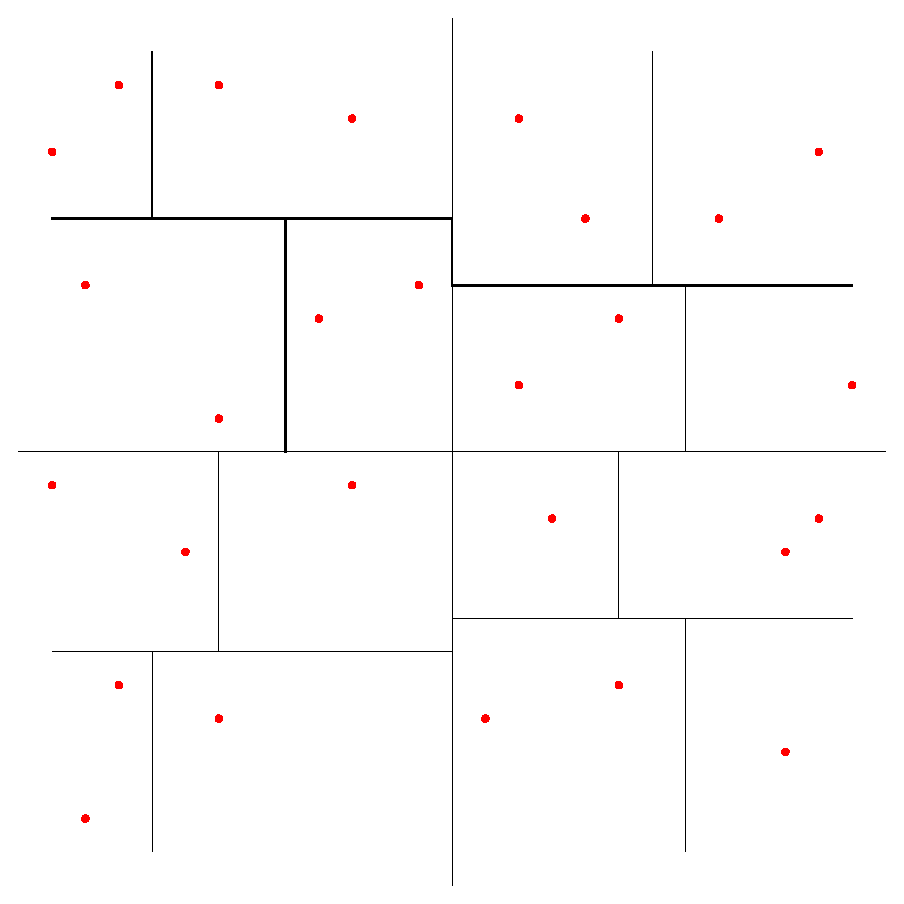
\includegraphics[width=8cm]{Figure1}
  \caption{Storing whole area covered by nodes}
  \label{fig:covered}
\end{figure}

Imagine that we want to find point with smallest value of the $x$ coordinate. We need to process all nodes
that don't have a lower bound on $x$. Lets count them:
\bigskip

$T(1) = 1$

$T(n) \geq 2^{d-1} * T(n/2^{d})$

\bigskip

There are $\Omega (n^{1-1/d})$ such nodes. Instead of storing whole area covered by the node (see Figure~\ref{fig:covered}), we could calculate area covered by points inside each node. 

 (Figure~\ref{fig:inside}).

\begin{figure}
\centering
  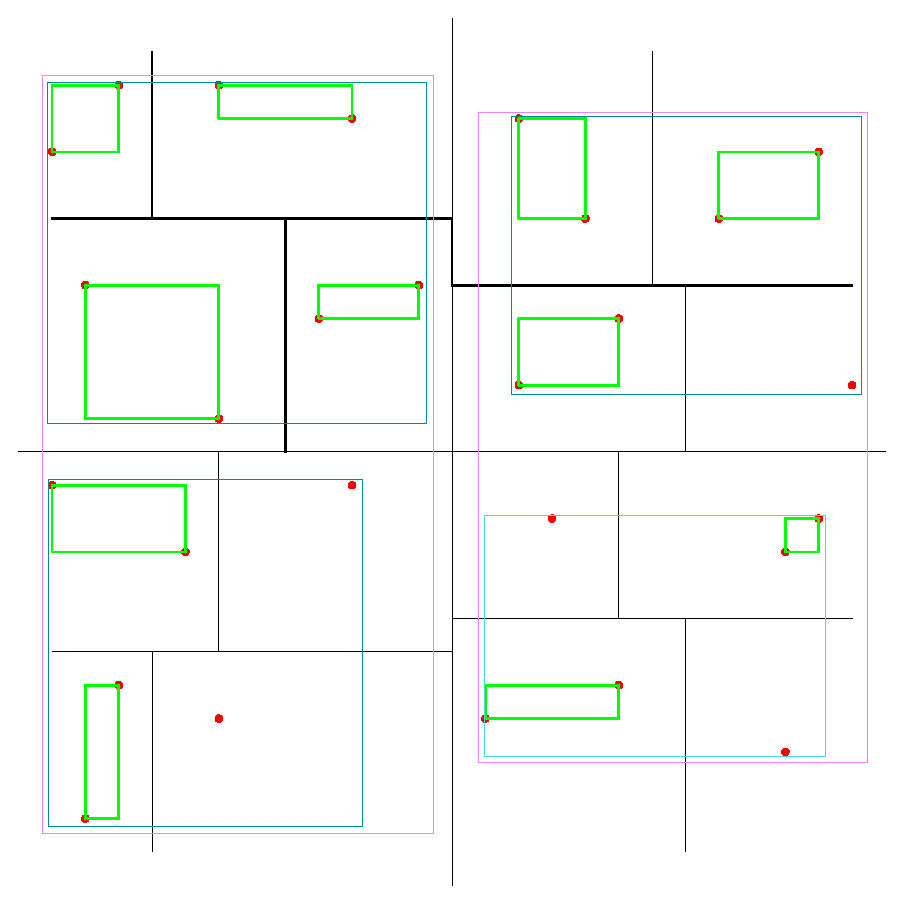
\includegraphics[width=8cm]{Figure2}
  \caption{Area covered by points inside nodes}
  \label{fig:inside}
\end{figure}

Lets revised this idea on example where point with minimal value of coordinate x is searched. First event contains root of a tree. It is processed. It causes to push two of its sons to the queue. Then we chose node with smaller minimum value of coordinate x. This event is processed and another two nodes are added. Point with minimal value of coordinate x belongs to exactly one of these nodes, and this node is processed. This situation goes on until leaf containing point with minimum value of coordinate x is processed. At this point we found point with minimal value of coordinate x. Search process can be stopped and results may be rendered. Summarizing $\Oh(\log n)$ nodes are added to queue, and $\Oh(\log n)$ are processed. Finding minimum value of coordinate x of node takes $O(1)$ since we are storing this information in boundary. Processing one node takes $\Oh(1)$ time. Bootleneck of this solution is priority queue. Priority queue may be implemented as a binary heap. We processed $\Oh(\log n)$ nodes so complexity of this solution is $\Oh(\log n \log \log n)$. It can be improved by using binomial heaps \cite{BINOMHEAPS}. Binomial heap has an insert in amortized time of $\Oh(1)$ and finding minimum in $\Oh(1)$ which reduces complexity to $\Oh(\log n)$.

\subsection{Raw pointers instead of shared pointers}

In modern C++ pointers shouldn't be used, and shared pointers are recommended instead. Idea behind shared pointer is to automate releasing resources. Basically shared pointer keeps counter representing the number of copies of current pointer. When shared pointer is created, counter is incremented. When shared pointer is deleted, then counter is decremented. When counter is down to zero, then resource is released. With such a tool, developer is free from most common cause of memory leaks. Unfortunately such tool comes with time and space overhead. I decided to use raw pointers which give better running and space time.
Right now I think it was biggest mistake in the project. Source code became really messy, even small change in legacy code could create bugs.

\subsection{Balancing K-D tree}
K-D tree has similar problem to binary trees. Binary tree can be unbalanced and so can K-D tree. My idea for balancing K-D tree is very simple. When number of nodes in one subtree is 5 times larger that number of nodes in opposite subtree, then I'm rebuilding their parent subtree from the beginning.
This is known as partial rebuilding, a simple yet very powerful paradigm often used for making data structures dynamic, for example in weight-balanced trees~\cite{ALPHATREES}. While the worst case complexity of a single operations can be large because of this rebalancing, the amortized complexity~\cite{AMOR} is actually rather good.


\section{Complexities}

Nomenklatura:
\begin{enumerate}
\item left($\theta$) - left subtree of vertex $\theta$
\item right($\theta$) - right subtree of vertex $\theta$
\end{enumerate}

Let $n$ be number of points in the tree. Tree is X-balanced if and only if \todo{for every vertex X w texu} X * |left($\theta$)| >= |right($\theta$)| $\wedge$ X * |left($\theta$)| >= |right($\theta$)|. Tree is well-balanced if it's 2-balanced. Tree is barely-balanced if it's 5-balanced. Height of both well and barely balanced trees are $\Oh(\log n)$. Every point belongs to $\Oh(\log n)$ nodes. 

Assumptions:
\begin{enumerate}
\item all values of all columns are unique
\item rebuilding subtree with root $\theta$ causes subtree with root $\theta$ to be well-balanced.
\end{enumerate}

\subsection{Inserting/deleting point $X$}

\pawel{Zwróć uwagę na to, że dowody są oznaczone jako dowody...}

\pawel{Tutaj używałeś S jako liczby, a potem pisałeś |S|?!}
\begin{lemma}\label{lem:1}
Rebuilding tree of size $n$ takes $\Oh(n \log n)$.
\end{lemma}

\begin{proof}
We can find the median in linear time~\cite{FIVE}. Hence in order to rebuild a tree, we first find the median, and then recursively rebuild two subtrees half the size. Complexity of such procedure can be described by $T(n) = 2 T(n/2) + \Oh(n)$, which solves to $T(n) = \Oh(n \log n).$
\end{proof}

\begin{lemma}\label{lem:2}
Amortized time of insert/delete is $\Oh(\log^2 n)$.
\end{lemma}

\begin{proof}

We will give $3\log n$ credits to each node visited during insert/delete. As the depth of the whole tree is $\Oh(\log n)$, the total number of credits allocated during a single insert/delete operation is just $\Oh(\log^{2}n)$. The goal is to make sure that the following invariant holds: a node such that the left subtree is of size $n_{l}$ and the right subtree is of size $n_{r}$ has at least $3|n_{l}-n_{r}|\log n$ credits available (observe that because the tree is well-balanced, this is at most $n\log n$). We must prove that the invariant still holds after each insert/delete and that we always have enough credits to amortize the rebuilding. We consider those two parts separately.

\begin{enumerate}

\item Each node visited during an insert/delete operation gets $3\log n$ credits. Notice that after the visit we either increase or decrease $n_{l}$ or $n_{r}$. Hence we increase $3|n_{l}-n_{r}|\log n$ by at most $3\log n$, and so we can afford to pay for this increase using the new credits allocated to the node (it can also happen that we decrease $|n_{l}-n_{r}|\log n$, which is even better).

\item We rebuild a node as soon as one subtree is five times larger than the other, say $n_{l} = 5n_{r}$. Then the number of credits accumulated at the node is at least ($n_{l}-2n_{r}
)\log n = 3n_{r}\log n \geq n\log n$, where $n=n_{l}+n_{r}$. After we reconstruct the tree, the required number of credits will be at most $\log n$. Hence we can use $(n-1)\log n$ credits to pay for the reconstruction, and by Lemma~\ref{lem:1} this is enough.

\end{enumerate}

There is one additional details. The value of $\log n$ can (and will) actually change during the execution of the algorithm. We actually care about its integer part, tough. In order for it to increase, we need to perform $n$ insert/delete operations. Hence if we charge each such operation with additional $c\log^{2} n$ credits, whenever the integer part of $\log n$ increases, we will have $cn\log^{2} n$ credits available. Now, for each node of the tree we need to add $n\log n$ credits, hence the total required number of credits is described by the recurrence $T(n)=n\log n+T(\alpha n)+T((1-\alpha)n)$, where $\frac{1}{3}\leq \alpha \leq \frac{2}{3}$. The recurrence solves to $T(n)=\Theta(n\log^{2}n)$ \pawel{proof?} \jarek{Teraz bym to indukcyjnie udowadniał, we Wrocławiu otworze konkretną i przypomne sobie jak się takie rzeczy robi} so we have enough credits to pay for the increase.
\end{proof}


\pawel{Tutaj fajnie byłoby skonstruować przykład, że ta złożoność to faktycznie $\log^{2}n$, tzn ciąg $n$ insertów, które w sumie wymagają czasu $n\log^{2}n$...}

\subsection{Search}
\pawel{Jak dla mnie to does change... mi wychodzi $\Oh(n^{1-1/d+\epsilon}+k)$, $\epsilon$ zależy jakoś od balansu między dziećmi}

Recall that the complexity of searching in a static K-D tree is $\Oh(n^{1-1/d} + k)$. The usual proof of such bound is by analyzing a query of the form $x>=c$. We want to bound the number of nodes whose cells intersect the boundary of such query. Because every $d$-th level of the tree partitions the points according to the $x$ coordinate, we can write the recurrence $T(n)=1+2^{d-1}T(\frac{n}{2^{d}})$, which by the master theorem solves to $T(n)=\Oh(n^{\frac{\log 2^{d-1}}{\log 2^{d}}})=\Oh(n^{1-1/d})$. 

Unfortunately, such worst case bound seems difficult to achieve in our dynamic settings, where the tree is just almost balanced. Nevertheless, a slightly weaker bound holds under the assumption that a child of a node corresponding to $n$ points corresponds to at most $\frac{2}{3}n$ points itself. Then the recurrence describing the worst-case behavior is $T(n)=1+2^{d-1}T(\frac{\frac{2}{3}n}{2^{d-1}})$ \pawel{uzasadnić!}, which (again by the master theorem) solves to $T(n)=\Oh(n^{\frac{\log 2^{d-1}}{\log 3*2^{d-2}}})=\Oh(n^{\frac{d-1}{d-0.42}})=\Oh(n^{1-0.58/(d-0.42)})$. \pawel{brzydki wynik}

\jarek{Uważasz, że pisanie o average casie ma sens? Taki fragment jest przydany, ale bez względu na to jak go napiszę, brzmi jak wyciąganie królika z kapelusza;/}
\pawel{Może i przydatny, tylko to explanation bym zmienił.  I dodał, że chodzi Ci o losowe punkty?}
\bigskip

While the worst case bound might seem somehow disappointing when $d$ is large, one should remember that in practice we will observe a much better performance. For average queries algorithm behaves like $\Oh(S \log n)$ where S = offset + limit. Explanation: when algorithm recursively enters node of K-D tree, then it usually finds some results. It means that finding single row, usually takes $\Oh(\log n)$.

\section{Tested engines}
\subsection{Solr}

Schema used in testing is:

\begin{verbatim}
<fields>
  <field name="id" type="uuid" indexed="true" stored="true" default="NEW"/>
   <field name="first_name" type="text_general" indexed="true"
             stored="true" required="true" /> 
   <field name="last_name" type="text_general" indexed="true" 
             stored="true" required="true"/>
   <field name="age" type="int" indexed="true" stored="true" /> 
   <field name="city" type="text_general" indexed="true" stored="true"/>
</fields>

<uniqueKey>id</uniqueKey> 
\end{verbatim}

Solr requires unique key. Combining all properties isn't enough. For example there are lots of guys named Jan Kowalski in Warsaw. Therefore I created another property named id.

Syntax: \todo{Nie pamietam czy w rangu syntax nie jest value:[from,to]}
\begin{enumerate}
\item Comparisons: \verb|property:value|
\item Inequalities are realized by range queries: \verb|property:[from to]|. \verb|From| and \verb|to| can be replaced by *. Number greater or equal to 2 can be searched by \verb|property:[2 *]|. \verb|property:[* *]| matches everything.
\item Prefix queries: \verb|property:value*|.
\item Substring queries: \verb|property:*value*|.
 
\end{enumerate}

\subsection{PostgreSQL}

Schema used in testing is: \todo {sprawdź czy dobrze to napisałeś}

\begin{verbatim}
CREATE TABLE users (
  first_name TEXT not null,
  last_name TEXT not null,
  age INT not null,
  city TEXT not null
);

CREATE INDEX index1 ON users (first_name, last_name, age, city);
CREATE INDEX index2 ON users (last_name, age, city);
CREATE INDEX index3 ON users (city, age, first_name);
CREATE INDEX index4 ON users (age, first_name, last_name);
\end{verbatim}

Syntax:
\begin{enumerate}
\item Comparisons and inequalities are realized by \verb|=|, \verb|>=|, \verb|>|, \verb|<=|, \verb|<|
\item Prefix queries are handled by \verb|property LIKE "text\%"|
\item Substring queries are handled by \verb|property LIKE "\%text\%"|
\end{enumerate}

For text-search PostgreSQL implemented special type of indexes: GIN \cite{PSQLGIN} and GIST \cite{PSQLGIST}. Unfortunately I was unsuccessful in making them work with polish words. Therefore I'm testing PostgreSQL with default indexes.

\section{Tested results}

\subsection{How results are tested}

Testing environment is machine with Intel i5-2500 processor (4 cores, 3.5GHz), 8GB RAM and SSD drive. Comparing engines with default settings is pointless. I've tried to configure them all to production use. Most important change is increased memory limit to 2GB (it seems 25 percent RAM capacity is recommended limit for all engines).

In nk we've got several millions registered users. This number doesn't grow in spectacular fashion. I wan't to simulate engines behaviour in similar conditions. 

At the beginning I'm inserting $8 * 10^6$ random users. Then I'm running a script which creates random insert/search queries. It sends created queries for few hours and calculates statistics (avg running time, maximal running time).

Inserted data is generated in a very simple way. I've gather lists of most popular first names and last names in Poland (with counts). Probability of selecting name is proportional to it's count. Age is selected with linear distribution from set $[5, 100]$.

Search queries are generated by this procedure:
\begin{enumerate}
\item Pick N - number of expressions in search query
\item Column in expression is selected from set [first name, last name, age, city]. Each of them has 25 percent chance to be chosen.
\item If selected column has int type (only age is an integer) then possible queries are comparison and inequalities. There are 1 comparison and 4 inequalities. Each of them has 20 percent chance to be chosen.
\item If selected column has string type then possible queries are comparison, inequalities, prefix queries and substring queries. Prefix and substring queries are having 25 percent chance to be chosen. Each of the comparison and inequalities has 10 percent chance to be chosen. Selected column is always compared to another string. This string is selected by selecting random word with 1 to 5 characters. First character is uppercase others are lowercase characters. 
\end{enumerate}

Then I'm selecting random column and I'm setting it as order by column. Then I'm choosing offset and limit from range $[0, 50]$.

\subsection{Inserting 8 million rows}

8 million rows. Average string contains 7 characters. It means that size of inserted data is about 250 MB. There is always some overhead in keeping data structures. It causes shuffla to use 6 GB RAM.

Inserting 8 million rows isn't most important part of testing. It is performed before production deployment and we are doing this part only once. I'm happy as long as indexing time doesn't last longer than a few hours. 

Shuffla inserts data with 1000 request per second. Using single inserts with other engines isn't so efficient. All considered engines are able to read csv file and import data from such file. This is the only way to import data within few hours.

\todo{Być może trzeba ten akapit wywalić, inserty są raczej nieciekawe}
Shuffla is superior in inserts. It is caused by very low time complexity of insert and small number of reads/writes to disk. Shuffla actually requires writes to append log and slow log file but these writes can be disabled. Other engines are running with similar speed of 150 request per second. Lets remember that Solr, PostgreSQL are based on index which is stored on disk. This results were expected. Lets remember that Apache Solr doesn't cause changes to appear in results right away, so it's score is overrated. 

\subsection{Search statistics}

\todo{Rysunki się tworzą:)}

\section{Summary}

Results are suggesting that Shuffla is best for this problem. Business requirements made us choose solr. Besides speed we should look into following criterions:

\begin{enumerate}

\item In nk we are not going to stop working on search engine after implementing basic version described in this paper. There are lots of possible improvements like: grouping people by city, sorting them by number of common friends etc. Best way can be estimated by A/B tests, or analysis of search history. Before implementing simple version of search engine it's difficult to choose best solution or even estimate their effectiveness. It's impossible to create perfect search engine in terms of result effectiveness. Google is improving it's search engine to this day. Shuffla offers nothing more than tools described in abstract of this paper. This cuts number of possible improvements to minimum. Solr offers much more features, most important are facets. \todo{Tu widze kilka przykładów featurów solra których nie ma shuffla}

\item Nk users are not only searching for other users. Often they are looking for groups, applications, games, events and many more. Maybe in the future we would like to store all user content is search engine. Also there are features which do not exists yet. Chosen search engine must be very flexible. 

\item Solr is tested in combat. Lot's of big website services are using Solr. Right now nobody is using shuffla. What will happen when something brakes in shuffla? Nk developers will have to fix it. Such operation costs a lot (not mention downtime caused by the crash). Solr is mature software. It has many stable versions tested by many people. It's less likely that Solr will crash due to a bug. Even then there are chances that someone already encountered the same problem and described workaround.

\end{enumerate}

After this discussion you may think that Shuffla is useless. I don't think it's useless. Shuffla fits great for smaller problems like searching through internet forum or blog. Solr or sphinx are requiring not easy installation and configuration. Installation of shuffla takes 2 minutes, creating table takes 10 seconds and searching is very easy. In short/simple projects having possibility of integrating search engine in less than 5 minutes is very welcome. Unfortunately shuffla is not software which fulfils requirements of big social website.

\section{Few words about Solr in nk}

\todo{Wkleje tu statsy solra produkcjynego, wywiady z adminami i takie tam}

%%%%%%%%%%%%%%%%%%%%%%%%%%%%%%%%%%%%%%%%%%%%%%%%%%

\bibliographystyle{abbrv}
\bibliography{biblio}

\end{document}

%%%%%%%%%%%%%%%%%%%%%%%%%%%%%%%%%%%%%%%%%%%%%%%%%%